
Let
\begin{align}
   \vec{A} = \myvec{2\\-1\\1} , \vec{B} = \myvec{1\\-3\\-5}, \vec{C} = \myvec{3\\-4\\-4} 
\end{align}

\begin{align}
     (\vec{B}-\vec{A})^\top(\vec{C}-\vec{A})&=\myvec{-1\ -2\ -6}\myvec{1\\-3\\-5}
     \\
& = 35 \ne 0
\\
     (\vec{A}-\vec{B})^\top(\vec{C}-\vec{B})&=\myvec{1\ 2\ 6}\myvec{2\\-1\\1}
\\
&= 6 \ne 0
\\
(\vec{A}-\vec{C})^\top(\vec{B}-\vec{C})&=\myvec{-1\ 3\ 5}\myvec{-2\\1\\-1}
\\
&= 0
\end{align}
Hence, $\triangle ABC$ is right angled at C as shown in Fig. \ref{aug/2/3plot}.
%
\begin{figure}[!h]
         \centering
         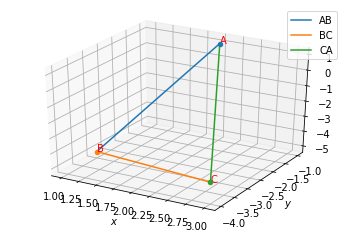
\includegraphics[width=\columnwidth]{solutions/aug/2/3/figures/right-angled.png}
         \caption{Plot of the triangle}
         \label{aug/2/3plot}
\end{figure}

